\documentclass[conference]{llncs}
\usepackage[english]{babel}
\usepackage[utf8]{inputenc}
\usepackage[T1]{fontenc}

\usepackage{times}
\usepackage{tikz-cd}
\usepackage{amssymb}
\usepackage{cite}
\usepackage{url}
\usepackage{listings}
\usepackage{tikz}
\usetikzlibrary{shapes,calc,positioning,arrows}
\usepackage{algorithm}
\usepackage{algorithmic}
\usepackage{paralist}
\usepackage{textcomp}
\def\BibTeX{{\rm B\kern-.05em{\sc i\kern-.025em b}\kern-.08em
    T\kern-.1667em\lower.7ex\hbox{E}\kern-.125emX}}

\usepackage{varioref}
\usepackage[pdfpagelabels=true]{hyperref}

\usepackage{amsmath}

\newcommand{\name}{BlindCons}

%\newtheorem{definition}{Definition}
%\newtheorem{theorem}{Theorem} 
%\newtheorem{proof}{Proof} 

\pagestyle{plain}
\newcounter{paranum}
\newcommand{\Par}{\vspace{10pt}\noindent\textbf{\refstepcounter{paranum}\theparanum}\textbf\textit) }

\begin{document}

\title{\name{}: A Consensus Algorithm for Privacy Preserving Private Blockchains\\}

%\author{Mirko Koscina$^{1,3}$ \and Pascal Lafourcade$^2$ \and David Manset$^3$ \and David Naccache$^1$}
%\institute{$^1$\'Ecole normale sup\'erieure\\
%45 rue d'Ulm, \textsc{f}-75230 Paris \textsc{cedex 05}, France\\
%\email{\url{given\_name.family\_name@ens.fr}} \\
%$^2$Universit\'e Clermont Auvergne\\
%LIMOS, UMR 6158, F-63173, France\\
%\email{\url{given\_name.family\_name@uca.fr}} \\
%$^3$Almerys\\
%46 Rue du Ressort, 63967 Clermont-Ferrand \textsc{cedex 9}, France\\
%\email{\url{given\_name.family\_name@almerys.com}}
%}

\maketitle


\begin{abstract}
Private blockchains are becoming gradually more sought-after in many organisations. Predominately because they allow organisations to overpass the traditional limitations of public blockchains in terms of energy consumption, efficiency, and control of the system. However, such systems are in some ways losing their blockchain essence, particularly their unique feature of not being controlled by a central authority that governs many functionalities of the chain including user enrolment. Our main contribution in this paper is to propose a user ID privacy preserving consensus algorithm for private blockchains, called \name{}. The main security properties of our protocol guarantee: consistency of the data stored in the blockchain, liveness of the system, and users' privacy by blinding their signatures to keep the user identity private. \name{} blind signature scheme ensures that it is not possible to link a transaction to a user using the data stored in the blockchain. Our consensus BlindCons uses Okamoto-Schnorr Blind Signature proposed in 1992 and a Byzantine Fault Tolerance (BFT) consensus for the blockchain replication process.
\end{abstract}

\keywords{blind signature, transactions unlinkability, privacy-preserving consensus,  permissionned blockchain.}

\section{Introduction} \label{intro}

Currently, blockchain is one of the most popular distributed systems. One of the main characteristics of blockchains is their resistance to malicious modifications. Such resistance is reached by using block timestamp and hash pointers that link the last block of the chain to the previous one. The blockchain design forces that any modification in one block compels the regeneration of the following blocks in the chain. A consensus algorithm controls the blockchains data storage process, ensuring that any update on the chain is valid and committed by all the network members.

Many groups of companies have proposed \emph{Private Blockchains} or \emph{Permissioned Blockchains}, like for instance the MyHealthMyData  consortium~\cite{MHMD}, which propose to connect hospitals and research centers across Europe to share medical data through a private blockchain network. These blockchains aim to manage data storage on a few nodes controlled by a company or a consortium in order to validate the transactions fastest, consume less energy and reduce the cost of mining. Another example is the project PlasticTwist~\cite{PTWIST} that creates a new circular economy based on an ERC20 token implemented on the top a permissioned ledger to encourage plastic recycling in Europe. Moreover, Maersk and IBM have developed TradeLens~\cite{Tradelens}, a supply chain system supported by the permissioned blockchain Hyperledger Fabric.  

Use cases, like the examples presented above, are proliferating due to the blockchain adoption in closed ecosystems and business applications. Due to this, the European Blockchain Observatory and Forum has published a technical report~\cite{BlockchainGDPR} where it recommends to use private or permissioned blockchains for storing sensitive data. Therefore, the absence of mechanisms to keep the user's privacy in a permissioned scheme is turning highly relevant.


\paragraph*{Contributions:} The main contribution of this paper is the design of a new privacy-preserving consensus algorithm for private blockchains. We aim to ensure the unlinkability between a transaction recorded in the blockchain and the user that generated it. With our algorithm, we increase the privacy level of such blockchains. For this purpose, we designed a privacy-preserving consensus called \name{}. Our algorithm relies on Okamoto-Schnorr's blind signature scheme~\cite{okamoto1992provably} to ensure transaction unlinkability. Moreover, we use a Byzantine Fault Tolerance (BFT) consensus algorithm for the generation and commitment of new blocks.


\paragraph*{Related Work:}
Blockchain platforms such as Bitcoin~\cite{nakamoto2008bitcoin} and Ethereum~\cite{wood2014ethereum} are popular due to the ``anonymity'' that their cryptocurrencies offer. However, Bitcoin is still showing issues with transaction linkability and traceability.  During the last years some improvements have been proposed to increase Bitcoin anonymity~\cite{saxena2014increasing}, and also new cryptocurrencies have been developed to overcome these issues like Zcash and Monero. In the case of Zcash ~\cite{hopwood2016zcash}, the protocol achieves anonymity by using ZK-SNARKs as cryptographic proof. In the same line, Bulletproofs~\cite{bunz2018bulletproofs} proposes a new NIZKP protocol with short proofs without relying on trusted setup for confidential transactions or privacy preserving smart contracts. On the other hand, Monero is a protocol based on Cryptonote~\cite{van2013cryptonote} that achieves unlinkability and untraceability by using a one-time random address and ring signatures.  Although all these protocols aim to improve transactions' privacy, they are designed for permissionless blockchains, where the transaction linkability differs from permssioned architecture where the users are not anonymous. Hence, there is a strong link between the transaction signature and the user that is triggering it.

A different approach to ensure anonymity is the eCash~\cite{chaum1983blind}~\cite{chaum1988untraceable} model proposed for Bitcoin in~\cite{heilman2016blindly}. However, the idea to use a third party to generate a blind voucher is not aligned with the principle of decentralisation that Bitcoin or any other permissionless blockchains have. 

Notwithstanding several works on blockchain privacy for permissionless ledgers have been published, as far as we know, there is no formal protocol that addresses the transaction linkability issue in permissioned ledgers

\paragraph*{Outline:}  Section~\ref{back} recalls Permissioned Blockchains and Okamoto-Schnorr's blind signature scheme, then in Section~\ref{PBFTHF} we introduce the BFT consensus mechanism. Section~\ref{PPPBFT} describes our privacy-preserving consensus algorithm \name{}. Before concluding, we explicit the security properties of our consensus algorithm in Section~\ref{PROP}.


\section{Preliminars} \label{back}

We start by introducing permissioned blockchains, and then we present a blind version of the Schnorr's signature scheme proposed by Okamoto et al. in~\cite{okamoto1992provably}.

\subsection{Permissioned Blockchain}
\label{Permissioned}
TODO

\subsection{Okamoto et al. Signature}
\label{Okamoto}

This scheme allows the user to obtain a blind signature of the message $M\in \{0,1\}^*$ issued by an authority ($A$). 

\begin{definition}[Okamoto-Schnorr Blind Signature~\cite{okamoto1992provably}]
Let $p$ and $q$ be two large primes with $q|p-1$. Let $G$ be a cyclic group of prime order $q$, and $g$ and $h$ be generators of $G$. Let $H:\{0,1\}^*\rightarrow \mathbb{Z}_q$ be a cryptographic hash function.
\begin{compactdesc}
\item[Key Generation:] Let $(r,s) \xleftarrow[]{r}\mathbb{Z}_q$ and $y=g^rh^s$ be the $A$'s private and public key, respectively.
\item[Blind signature protocol:]
\begin{compactenum}
    \item $A$ chooses $(t,u) \xleftarrow[]{r}\mathbb{Z}_q$, computes $a = g^th^u$, and sends $a$ to the user.
    \item The user chooses $(\beta, \gamma, \delta) \xleftarrow[]{r}\mathbb{Z}_q$ and computes the blinded version of $a$ as $\alpha=ag^{-\beta} h^{-\gamma} y^\delta$, and $\epsilon=H(M,\alpha)$. Then calculates $e=\epsilon-\delta$ mod $q$, and sends $e$ to the $A$.
    \item $A$ computes $S=u-es$ mod $q$ and $R=t-er$ mod $q$, sends $(S,R)$ to the user.
    \item The user calculates $\rho=R-\beta$ mod $q$ and $\sigma=S-\gamma$ mod $q$.
\end{compactenum}
\item[Verification:] Given a message $M\in \{0,1\}^*$ and a signature $(\rho,\sigma,\epsilon)$, we have $\alpha=g^\rho h^\sigma y^\epsilon$ mod $p$.
\end{compactdesc}
\end{definition}

\begin{figure*}[tb]
\centering
\fbox{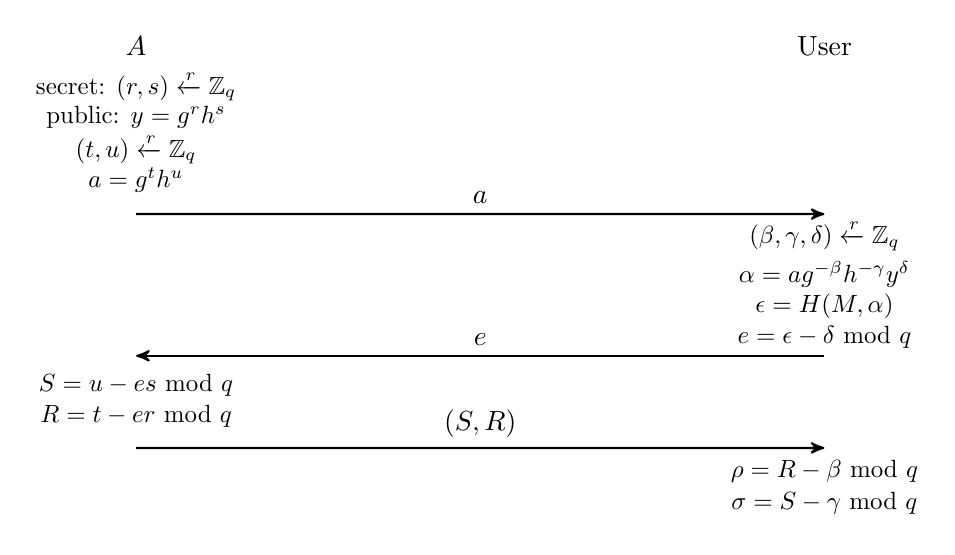
\begin{tikzpicture}[node distance=8cm,auto,>=stealth',scale=1,thick]
    \node[] (user) {User};
    \node[left = of user] (ca) {$A$};
    \node[below of=ca,scale=0.9, node distance=0.5cm] (ca_l1r1) {secret: $(r,s) \xleftarrow[]{r}\mathbb{Z}_q$};
    \node[below of=ca_l1r1,scale=0.9, node distance=0.4cm] (ca_l2r1) {public: $y=g^rh^s$};
    \node[below of=ca_l2r1,scale=0.9, node distance=0.4cm] (ca_l3r1) {$(t,u) \xleftarrow[]{r}\mathbb{Z}_q$};
    \node[below of=ca_l3r1,scale=0.9, node distance=0.4cm] (ca_l4r1) {$a = g^th^u$};
    \node[below of=ca_l4r1,scale=0.9, node distance=2cm] (ca_l1r3) {};
    \node[below of=ca_l1r3,scale=0.9, node distance=0.6cm] (ca_l2r3) {$S=u-es$ mod $q$};
    \node[below of=ca_l2r3,scale=0.9, node distance=0.4cm] (ca_l3r3) {$R=t-er$ mod $q$};
    \node[below of=ca_l3r3,scale=0.9, node distance=0.3cm] (ca_l4r3) {};
    \node[below of=ca,scale=0.9, node distance=6cm] (ca_ground) {};
    \node[below of=user,scale=0.9, node distance=1.7cm] (user_l1r2) {};
    \node[below of=user_l1r2,scale=0.9, node distance=0.7cm] (user_l2r2) {$(\beta, \gamma, \delta) \xleftarrow[]{r}\mathbb{Z}_q$};
    \node[below of=user_l2r2,scale=0.9, node distance=0.5cm] (user_l3r2) {$\alpha=ag^{-\beta} h^{-\gamma} y^\delta$};
    \node[below of=user_l3r2,scale=0.9, node distance=0.4cm] (user_l4r2) {$\epsilon=H(M,\alpha)$};
    \node[below of=user_l4r2,scale=0.9, node distance=0.4cm] (user_l5r2) {$e=\epsilon-\delta$ mod $q$};
    \node[below of=user_l5r2,scale=0.9, node distance=1.3cm] (user_l1r4) {};
    \node[below of=user_l1r4,scale=0.9, node distance=0.4cm] (user_l2r4) {$\rho=R-\beta$ mod $q$};
    \node[below of=user_l2r4,scale=0.9, node distance=0.4cm] (user_l3r4) {$\sigma=S-\gamma$ mod $q$};
    \node[below of=user,scale=0.9, node distance=6cm] (user_ground) {};
    %

    \draw[->] ($(ca_l4r1)!0.1!(ca_ground)$) -- node[above,scale=1,midway]{$a$} ($(user_l1r2)!0.1!(user_ground)$);
    \draw[<-] ($(ca_l1r3)!0.1!(ca_ground)$) -- node[above,scale=1,midway]{$e$} ($(user_l5r2)!0.1!(user_ground)$);
    \draw[->] ($(ca_l4r3)!0.1!(ca_ground)$) -- node[above,scale=1,midway]{$(S,R)$} ($(user_l1r4)!0.1!(user_ground)$);
\end{tikzpicture}}
\caption{Okamoto-Schnorr blind signature diagram, where $y \xleftarrow[]{r}\mathbb{Z}_q$ means that $y$ is randomly chosen in $\mathbb{Z}_q$.}
\label{dia:oss}
\end{figure*}

The Okamoto-Schnorr blind signature scheme is suitable for private blockchain architecture due to the blinding process can be performed by the same authority responsible for the enrollment process (see Figure~\ref{dia:oss}, where the authority $A$ blinds the signature of the message proposed by the user). Therefore, by using this scheme, we ensure user-transaction unlinkability.

\section{Byzantine Fault Tolerant based Consensus for Private Blockchain Architecture}
\label{PBFTHF}

The blockchain is a decentralised database organised in blocks that are appended one behind the other by using a hash pointer. Each block contains records that include the data to be stored into the chain. The blockchain design makes it suitable to be used as a distributed ledger, due to the record organisation inside a block (i.e., financial transactions) and the hash chain between blocks that makes it resistant to malicious modifications. The blockchain uses a consensus algorithm to replicate the chain in each node member of the network. Nevertheless, the selection or design of the consensus algorithm must be consistent with the blockchain architecture and the openness of the system.

In permissioned blockchain architectures, every user must be enrolled into the system through Certificate Authorities (CA) or user administrators before joining the network. These authorities are responsible for generating the user credential for each new client or peer. This model provides a base of knowledge of the network members, making PBFT~\cite{castro1999practical} or BFT-Smart~\cite{6903593} based algorithms suitable for the blockchain replication process.  

Our consensus approach for permissioned ledger has an opposite aim of the permissionless replication protocol. The security of the consensus algorithm in a permissionless architecture is achieved by proving the node's honesty by expending its resources (i.e., computing capacity, power consumption, stakes, among others). In contrast, a BFT-based protocols reach the consensus accepting as valid the result proposed by the nodes majority. 

Our consensus algorithm is based on BFT and the \textit{execute-order-validate} process used in Hyperledger Fabric~\cite{androulaki2018hyperledger} since version 1.0. In this protocol, each transaction passes through these three stages. The \textit{execution} phase triggers the transaction and then it is validated by endorsement. In the \textit{order} phase, the transactions are ordered according to the BFT consensus protocol. Finally, the \textbf{validation} phase checks the security policies per operation and application types.

In the case of our BFT-based consensus algorithms, we start with a client $c_{bc}$ that has the same role than a client in the PBFT protocol. The client $c_{bc}$ sends a transaction proposal with the instructions to be executed in the blockchain to the endorsing peers in order to validate the transaction. This process is analogous than the executed by the primary in the original PBFT algorithm, that sends the message with the instructions to the backups to validate it. As for the transaction endorsement, the endorsing peers $ep_{bc_{i}}$ send their responses to the client, which collects it after the validation process is concluded. If the transaction is valid, the client $c_{bc}$ sends the transaction to the orderers $ordp_{bc_{i}}$ to add it into the new block that will be committed by the nodes members of the network. The orderes are responsible to propose and agreed the new block to be appended to the chain. This process is analogous to PBFT, where one orderer is the leader and the other are the backups. The orderer leader will collect a group of transactions and will organise them by order inside of a new block. Then the orderer leader sends the block proposal to the orderers backups to validate it. Each orderer backup will validate the proposal and responds to the rest of the orderer with a \textbf{prepare} message. Once the orderers have received enough valid \textbf{prepare} responses, they will submit a \textbf{commit} messages to the orderers, client and the nodes responsible to keep a local version of the blockchain. 

To exemplify this process, consider that we have a client $c_{bc}$ that needs to execute an operation $o_{bc}$ on our BFT-based blockchain protocol. To process this request, we need to execute the following four steps: Transaction Proposal, Transaction Endorsement, Broadcasting to Consensus and Commitment (see Figure~\ref{dia:pbft_BC}). Nevertheless,  before we start describing the protocol, we introduce the notation used in this paper. In any distributed system, the information is passing through the peers or nodes within the network by using messages. Hence, we  denote a message by using $<\cdot,...,\cdot>$, where $\cdot$ corresponds to the message arguments. Moreover, we use the notation $(\cdot,...,\cdot)$ to group arguments inside a message.

\begin{figure*}[tb]
\centering
\fbox{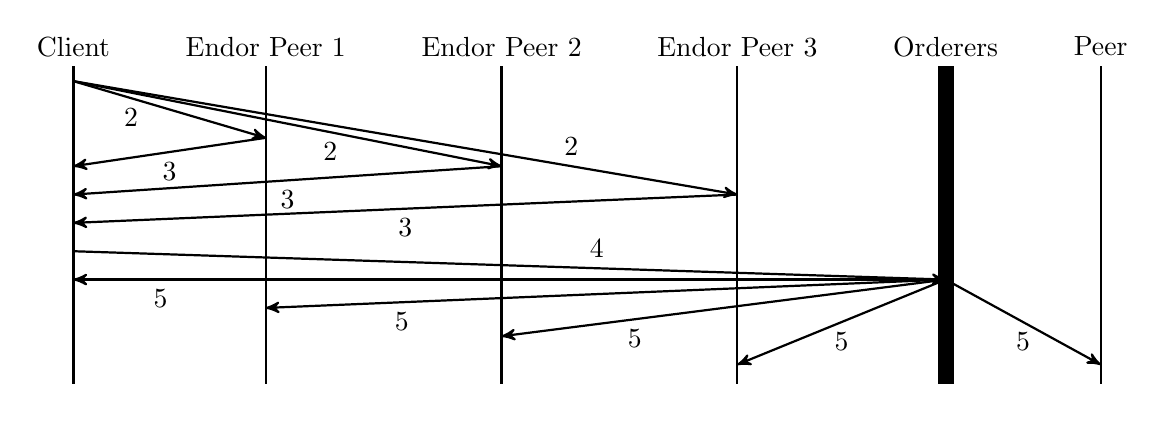
\begin{tikzpicture}[node distance=0.7cm,auto,>=stealth',scale=1,thick]
    %Nodes definition
    \node[scale=1] (peer) {Peer};
    \node[left = of peer, scale=1] (ord) {Orderers};
    \node[left = of ord, scale=1] (endp3) {Endor Peer 3};
    \node[left = of endp3,scale=1] (endp2) {Endor Peer 2};
    \node[left = of endp2,scale=1] (endp1) {Endor Peer 1};
    \node[left = of endp1, scale=1] (sp) {Client};
   % \node[left = of sp, scale=0.83] (client) {Client};
    %\node[below of=client,scale=0.9, node distance=0.4cm] (client1) {};
    %\node[below of=client1,scale=0.9, node distance=0.4cm] (client2) {};
    %\node[below of=client2,scale=0.9, node distance=0.4cm] (client3) {};
    %\node[below of=client3,scale=0.9, node distance=0.4cm] (client4) {};
    %\node[below of=client4,scale=0.9, node distance=0.4cm] (client5) {};
    %\node[below of=client5,scale=0.9, node distance=0.4cm] (client6) {};
    %\node[below of=client6,scale=0.9, node distance=0.4cm] (client7) {};
    %\node[below of=client7,scale=0.9, node distance=0.4cm] (client8) {};
    %\node[below of=client8,scale=0.9, node distance=0.4cm] (client9) {};
    %\node[below of=client9,scale=0.9, node distance=0.4cm] (client10) {};
    %\node[below of=client10,scale=0.9, node distance=0.4cm] (client_ground) {};
    \node[below of=sp,scale=0.9, node distance=0.4cm] (sp1) {};
    \node[below of=sp1,scale=0.9, node distance=0.4cm] (sp2) {};
    \node[below of=sp2,scale=0.9, node distance=0.4cm] (sp3) {};
    \node[below of=sp3,scale=0.9, node distance=0.4cm] (sp4) {};
    \node[below of=sp4,scale=0.9, node distance=0.4cm] (sp5) {};
    \node[below of=sp5,scale=0.9, node distance=0.4cm] (sp6) {};
    \node[below of=sp6,scale=0.9, node distance=0.4cm] (sp7) {};
    \node[below of=sp7,scale=0.9, node distance=0.4cm] (sp8) {};
    \node[below of=sp8,scale=0.9, node distance=0.4cm] (sp9) {};
    \node[below of=sp9,scale=0.9, node distance=0.4cm] (sp10) {};
    \node[below of=sp10,scale=0.9, node distance=0.4cm] (sp_ground) {};
    \node[below of=endp1,scale=0.9, node distance=0.4cm] (endp11) {};
    \node[below of=endp11,scale=0.9, node distance=0.4cm] (endp12) {};
    \node[below of=endp12,scale=0.9, node distance=0.4cm] (endp13) {};
    \node[below of=endp13,scale=0.9, node distance=0.4cm] (endp14) {};
    \node[below of=endp14,scale=0.9, node distance=0.4cm] (endp15) {};
    \node[below of=endp15,scale=0.9, node distance=0.4cm] (endp16) {};
    \node[below of=endp16,scale=0.9, node distance=0.4cm] (endp17) {};
    \node[below of=endp17,scale=0.9, node distance=0.4cm] (endp18) {};
    \node[below of=endp18,scale=0.9, node distance=0.4cm] (endp19) {};
    \node[below of=endp19,scale=0.9, node distance=0.4cm] (endp110) {};
    \node[below of=endp110,scale=0.9, node distance=0.4cm] (endp1_ground) {};
    \node[below of=endp2,scale=0.9, node distance=0.4cm] (endp21) {};
    \node[below of=endp21,scale=0.9, node distance=0.4cm] (endp22) {};
    \node[below of=endp22,scale=0.9, node distance=0.4cm] (endp23) {};
    \node[below of=endp23,scale=0.9, node distance=0.4cm] (endp24) {};
    \node[below of=endp24,scale=0.9, node distance=0.4cm] (endp25) {};
    \node[below of=endp25,scale=0.9, node distance=0.4cm] (endp26) {};
    \node[below of=endp26,scale=0.9, node distance=0.4cm] (endp27) {};
    \node[below of=endp27,scale=0.9, node distance=0.4cm] (endp28) {};
    \node[below of=endp28,scale=0.9, node distance=0.4cm] (endp29) {};
    \node[below of=endp29,scale=0.9, node distance=0.4cm] (endp210) {};
    \node[below of=endp210,scale=0.9, node distance=0.4cm] (endp2_ground) {};
    \node[below of=endp3,scale=0.9, node distance=0.4cm] (endp31) {};
    \node[below of=endp31,scale=0.9, node distance=0.4cm] (endp32) {};
    \node[below of=endp32,scale=0.9, node distance=0.4cm] (endp33) {};
    \node[below of=endp33,scale=0.9, node distance=0.4cm] (endp34) {};
    \node[below of=endp34,scale=0.9, node distance=0.4cm] (endp35) {};
    \node[below of=endp35,scale=0.9, node distance=0.4cm] (endp36) {};
    \node[below of=endp36,scale=0.9, node distance=0.4cm] (endp37) {};
    \node[below of=endp37,scale=0.9, node distance=0.4cm] (endp38) {};
    \node[below of=endp38,scale=0.9, node distance=0.4cm] (endp39) {};
    \node[below of=endp39,scale=0.9, node distance=0.4cm] (endp310) {};
    \node[below of=endp310,scale=0.9, node distance=0.4cm] (endp3_ground) {};
    \node[below of=ord,scale=0.9, node distance=0.4cm] (ord1) {};
    \node[below of=ord1,scale=0.9, node distance=0.4cm] (ord2) {};
    \node[below of=ord2,scale=0.9, node distance=0.4cm] (ord3) {};
    \node[below of=ord3,scale=0.9, node distance=0.4cm] (ord4) {};
    \node[below of=ord4,scale=0.9, node distance=0.4cm] (ord5) {};
    \node[below of=ord5,scale=0.9, node distance=0.4cm] (ord6) {};
    \node[below of=ord6,scale=0.9, node distance=0.4cm] (ord7) {};
    \node[below of=ord7,scale=0.9, node distance=0.4cm] (ord8) {};
    \node[below of=ord8,scale=0.9, node distance=0.4cm] (ord9) {};
    \node[below of=ord9,scale=0.9, node distance=0.4cm] (ord10) {};
    \node[below of=ord10,scale=0.9, node distance=0.4cm] (ord_ground) {};
    \node[below of=peer,scale=0.9, node distance=0.4cm] (peer1) {};
    \node[below of=peer1,scale=0.9, node distance=0.4cm] (peer2) {};
    \node[below of=peer2,scale=0.9, node distance=0.4cm] (peer3) {};
    \node[below of=peer3,scale=0.9, node distance=0.4cm] (peer4) {};
    \node[below of=peer4,scale=0.9, node distance=0.4cm] (peer5) {};
    \node[below of=peer5,scale=0.9, node distance=0.4cm] (peer6) {};
    \node[below of=peer6,scale=0.9, node distance=0.4cm] (peer7) {};
    \node[below of=peer7,scale=0.9, node distance=0.4cm] (peer8) {};
    \node[below of=peer8,scale=0.9, node distance=0.4cm] (peer9) {};
    \node[below of=peer9,scale=0.9, node distance=0.4cm] (peer10) {};
    \node[below of=peer10,scale=0.9, node distance=0.4cm] (peer_ground) {};

    % Vertical Lines
    %\draw (client) -- (client_ground);
    \draw (sp) -- (sp_ground);
    \draw (endp1) -- (endp1_ground);
    \draw (endp2) -- (endp2_ground);
    \draw (endp3) -- (endp3_ground);
    \draw[line width=0.2cm] (ord) -- (ord_ground);
    \draw (peer) -- (peer_ground);

    %Initiating Transactions
  %  \draw[->] ($(client)!0.1!(client_ground)$) -- node[below,scale=1,midway]{$1$} ($(sp)!0.1!(sp_ground)$);
    %Transaction Proposal
    \draw[->] ($(sp)!0.1!(sp_ground)$) -- node[below,scale=1,pos=0.3]{$2$} ($(endp12)!0.1!(endp1_ground)$);
    \draw[->] ($(sp)!0.1!(sp_ground)$) -- node[below,scale=1,pos=0.6]{$2$} ($(endp23)!0.1!(endp2_ground)$);
    \draw[->] ($(sp)!0.1!(sp_ground)$) -- node[above,scale=1,near end]{$2$} ($(endp34)!0.1!(endp3_ground)$);

    %Endorsing Transactions
    \draw[->] ($(endp12)!0.1!(endp1_ground)$) -- node[below,scale=1,midway]{$3$} ($(sp3)!0.1!(sp_ground)$);
    \draw[->] ($(endp23)!0.1!(endp2_ground)$) -- node[below,scale=1,midway]{$3$} ($(sp4)!0.1!(sp_ground)$);
    \draw[->] ($(endp34)!0.1!(endp3_ground)$) -- node[below,scale=1,midway]{$3$} ($(sp5)!0.1!(sp_ground)$);
    %Broadcasting to Consensus
    \draw[->] ($(sp6)!0.1!(sp_ground)$) -- node[above,scale=1,pos=0.6]{$4$} ($(ord7)!0.1!(ord_ground)$);
    %Commit
    \draw[->] ($(ord7)!0.1!(ord_ground)$) -- node[below,scale=1,pos=0.9]{$5$} ($(sp7)!0.1!(sp_ground)$);
    \draw[->] ($(ord7)!0.1!(ord_ground)$) -- node[below,scale=1,pos=0.8]{$5$} ($(endp18)!0.1!(endp1_ground)$);
    \draw[->] ($(ord7)!0.1!(ord_ground)$) -- node[below,scale=1,pos =0.7]{$5$} ($(endp29)!0.1!(endp2_ground)$);
    \draw[->] ($(ord7)!0.1!(ord_ground)$) -- node[below,scale=1,midway]{$5$} ($(endp310)!0.1!(endp3_ground)$);
    \draw[->] ($(ord7)!0.1!(ord_ground)$) -- node[below,scale=1,midway]{$5$} ($(peer10)!0.1!(peer_ground)$);
    
\end{tikzpicture}}
\caption{\name{} Transaction Flow.}
\label{dia:pbft_BC}
\end{figure*}

\Par{\textit{\textbf{Transaction Proposal:}}}
The client $c_{bc}$ generates a message to execute specific operations $o_{bc}$ to be resolved by the network. This message corresponds to a transaction proposal message to be sent to the endorsing peer. The transaction proposal consists in invoking the operations $o_{bc}$ and computing the state update and version dependency denoted by \textit{stateUpdate} and $\textit{verDep}$, respectively. The version dependencies relate the variables involve in the transaction with the local version of the variable in the client's node and their respective operations. For example: if a client wants to read and write in the blockchain, the version dependency is a tuple $\left(readset,writeset\right)$ where:

\begin{compactitem}
\item for every variable $k$ read by the transaction, the pair $(k,s(k).version)$ is added to readset,
\item for every variable $k$ modified by the transaction, the pair $(k,s(k).version)$ is added to $writeset$.
\end{compactitem}

Once the execution of the operations $o_{bc}$ triggered by the client $c_{bc}$ is completed, the client $c_{bc}$ generates the \textit{transaction proposal} message and then submits it to the endorsing peers. The transaction proposal message is defined as:

\noindent\fbox{\begin{minipage}[c]{0.98\textwidth}
$<\textit{PROPOSAL},trans_{prop}>$, where:
\begin{compactitem}
\item $trans_{prop}$:= $(c_{bc},o_{bc},txPayload,stateUpdate,$ $verDep, retryFlag, \sigma_c)$.
\begin{compactitem}
\item $c_{bc}$: is the client ID,
\item $o_{bc}$: refers to the operations implemented in the distributed system,
\item $txPayload$: is the payload of the submitted transaction,
\item $retryFlag$: boolean variable to identify whether to retry the transaction submission in case of the transaction fails, 
\item $\sigma_c$: is the client signature.
\end{compactitem}
\end{compactitem}
\end{minipage}}

\Par{\textit{\textbf{Transaction Endorsement:}}} The endorsing peers ($ep_{bc_{i}}$) verifies the client signature $\sigma_c$ coming in transaction proposal message. If the client signature is valid, the endorser simulates the transaction proposal by executing the operation $o_{bc}$ with the corresponding $txPayload$, and then validates that the $stateUpdate$ and $verDep$ are correct. If the validation process is successful, the endorsing peer generates a \textit{transaction valid} message to be sent to the client $c_{bc}$. The message has the following structure: ~\\

\noindent\fbox{\begin{minipage}[c]{0.98\textwidth}
$<\textit{TRANSACTION-VALID},tx_{id},\sigma_{ep_{i}}>$, where:
\begin{compactitem}
\item $tx_{id}$: is the transaction identifier generated with the client ID and a nonce,
\item $\sigma_{ep_{i}}$: is the signature of the message signed by the client $c_{bc}$.
\end{compactitem}
\end{minipage}}

In the case of the simulation process ending unsuccessfully, the endorsing peer generates a \textit{transaction invalid} message: ~\\

\noindent\fbox{\begin{minipage}[c]{0.98\textwidth}
$<\textit{TRANSACTION-INVALID},tx_{id},Error,\sigma_{ep_{i}}>$, where \textit{Error} can be:
\begin{compactitem}
\item \textit{INCORRECT-STATE}: when the endorser obtains a different \textit{state update} than the one coming in the \textit{transaction proposal},
\item \textit{INCORRECT-VERSION}: when there is the newest version of the variable referred in the \textit{transaction proposal},
\item \textit{REJECTED}: for any other reason.
\end{compactitem}
\end{minipage}}

\Par{\textit{\textbf{Broadcasting to Consensus:}}} The client $c_{bc}$ waits then for the response from the endorsing peers. When it receives enough \textit{Transaction Valid} messages adequately signed, the client stores the endorsing signatures into packaged called \textit{endorsement}. Once the transaction is considered endorsed, the client invokes the consensus services by using \textit{broadcast(blob)}, where \textit{blob:=(trans\textsubscript{prop}}, \textit{endorsement)}.

The number of valid responses needed to consider that the \textit{transaction proposal} is endorsed depends on the configuration of the permissioned blockchain. If the transaction has failed to collect enough endorsements, the client abandons this transaction proposal.

\Par{\textit{\textbf{Commitment:}}} Once the client $c_{bc}$ broadcasts the transaction properly endorsed to consensus, the ordering services collect this transaction and organise it into a block. The ordering service is sorted in \textit{views}, where each \textit{view} represents how the orderders are arranged for the consensus service. In each \textit{view}, the orderer $ordp_{leader}$ acts as the primary or leader, and the rest of the orderers ($ordp_{bc_{i}}; i=1,\cdots,n-1$) corresponds to the backups. In the case that the primary is faulty or is acting maliciously, the view will change and the next backup on the list will turn in the new leader. The consensus process begins when the orderer leader, $ordp_{leader}$, collects enough transactions to create a new block. The leader will propose this new block to the backups by sending a \emph{propose} message. Each backup validates the \emph{propose} and will respond to the other backups in the service with a message called \emph{prepare}. Once each backup has received enough valid \emph{prepare} responses, it will send a \emph{commit} message to nodes connected to the network to confirm that the block has been validated successfully. 

\begin{figure*}[tb]
\centering
\fbox{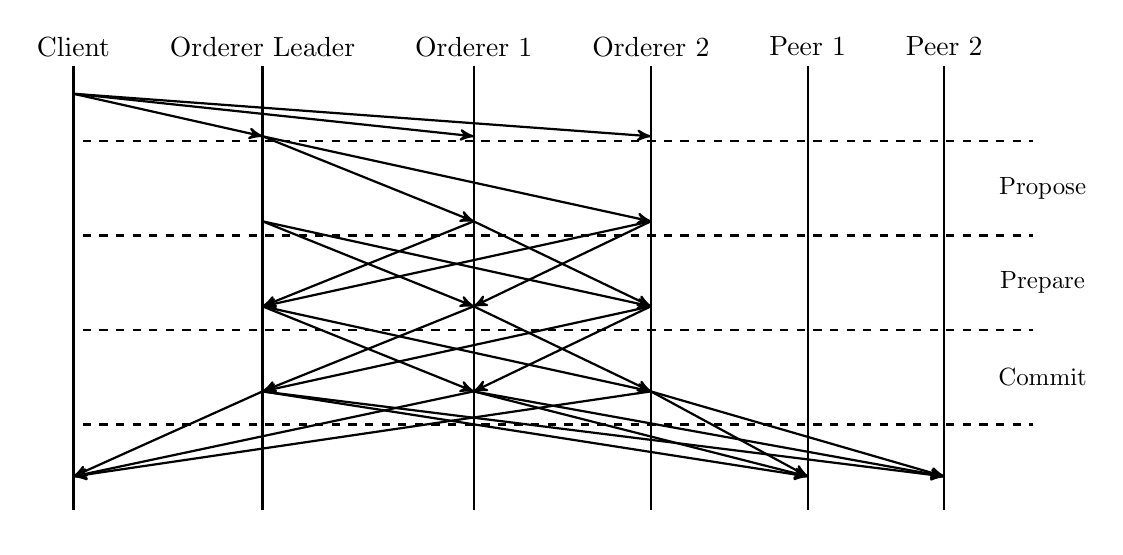
\begin{tikzpicture}[node distance=0.5cm,auto,>=stealth',scale=1,thick]
    %Nodes definition
    \node[scale=1] (comm) {};
    \node[left = of comm, scale=1] (peer) {Peer 2};
    \node[left = of peer, scale=1] (ord) {Peer 1};
    \node[left = of ord, scale=1] (endp3) {Orderer 2};
    \node[left = of endp3,scale=1] (endp2) {Orderer 1};
    \node[left = of endp2,scale=1] (endp1) {Orderer Leader};
    \node[left = of endp1, scale=1] (sp) {Client};
    
    \node[below of=sp,scale=0.9, node distance=0.6cm] (sp1) {};
    \node[below of=sp1,scale=0.9, node distance=0.6cm] (sp2) {};
    \node[below of=sp2,scale=0.9, node distance=0.6cm] (sp3) {};
    \node[below of=sp3,scale=0.9, node distance=0.6cm] (sp4) {};
    \node[below of=sp4,scale=0.9, node distance=0.6cm] (sp5) {};
    \node[below of=sp5,scale=0.9, node distance=0.6cm] (sp6) {};
    \node[below of=sp6,scale=0.9, node distance=0.6cm] (sp7) {};
    \node[below of=sp7,scale=0.9, node distance=0.6cm] (sp8) {};
    \node[below of=sp8,scale=0.9, node distance=0.6cm] (sp9) {};
    \node[below of=sp9,scale=0.9, node distance=0.6cm] (sp_ground) {};
    
    \node[below of=endp1,scale=0.9, node distance=0.6cm] (endp11) {};
    \node[below of=endp11,scale=0.9, node distance=0.6cm] (endp12) {};
    \node[below of=endp12,scale=0.9, node distance=0.6cm] (endp13) {};
    \node[below of=endp13,scale=0.9, node distance=0.6cm] (endp14) {};
    \node[below of=endp14,scale=0.9, node distance=0.6cm] (endp15) {};
    \node[below of=endp15,scale=0.9, node distance=0.6cm] (endp16) {};
    \node[below of=endp16,scale=0.9, node distance=0.6cm] (endp17) {};
    \node[below of=endp17,scale=0.9, node distance=0.6cm] (endp18) {};
    \node[below of=endp18,scale=0.9, node distance=0.6cm] (endp19) {};
    \node[below of=endp19,scale=0.9, node distance=0.6cm] (endp1_ground) {};
    
    \node[below of=endp2,scale=0.9, node distance=0.6cm] (endp21) {};
    \node[below of=endp21,scale=0.9, node distance=0.6cm] (endp22) {};
    \node[below of=endp22,scale=0.9, node distance=0.6cm] (endp23) {};
    \node[below of=endp23,scale=0.9, node distance=0.6cm] (endp24) {};
    \node[below of=endp24,scale=0.9, node distance=0.6cm] (endp25) {};
    \node[below of=endp25,scale=0.9, node distance=0.6cm] (endp26) {};
    \node[below of=endp26,scale=0.9, node distance=0.6cm] (endp27) {};
    \node[below of=endp27,scale=0.9, node distance=0.6cm] (endp28) {};
    \node[below of=endp28,scale=0.9, node distance=0.6cm] (endp29) {};
    \node[below of=endp29,scale=0.9, node distance=0.6cm] (endp2_ground) {};
    
    \node[below of=endp3,scale=0.9, node distance=0.6cm] (endp31) {};
    \node[below of=endp31,scale=0.9, node distance=0.6cm] (endp32) {};
    \node[below of=endp32,scale=0.9, node distance=0.6cm] (endp33) {};
    \node[below of=endp33,scale=0.9, node distance=0.6cm] (endp34) {};
    \node[below of=endp34,scale=0.9, node distance=0.6cm] (endp35) {};
    \node[below of=endp35,scale=0.9, node distance=0.6cm] (endp36) {};
    \node[below of=endp36,scale=0.9, node distance=0.6cm] (endp37) {};
    \node[below of=endp37,scale=0.9, node distance=0.6cm] (endp38) {};
    \node[below of=endp38,scale=0.9, node distance=0.6cm] (endp39) {};
    \node[below of=endp39,scale=0.9, node distance=0.6cm] (endp3_ground) {};
    
    \node[below of=ord,scale=0.9, node distance=0.6cm] (ord1) {};
    \node[below of=ord1,scale=0.9, node distance=0.6cm] (ord2) {};
    \node[below of=ord2,scale=0.9, node distance=0.6cm] (ord3) {};
    \node[below of=ord3,scale=0.9, node distance=0.6cm] (ord4) {};
    \node[below of=ord4,scale=0.9, node distance=0.6cm] (ord5) {};
    \node[below of=ord5,scale=0.9, node distance=0.6cm] (ord6) {};
    \node[below of=ord6,scale=0.9, node distance=0.6cm] (ord7) {};
    \node[below of=ord7,scale=0.9, node distance=0.6cm] (ord8) {};
    \node[below of=ord8,scale=0.9, node distance=0.6cm] (ord9) {};
    \node[below of=ord9,scale=0.9, node distance=0.6cm] (ord_ground) {};
    
    \node[below of=peer,scale=0.9, node distance=0.6cm] (peer1) {};
    \node[below of=peer1,scale=0.9, node distance=0.6cm] (peer2) {};
    \node[below of=peer2,scale=0.9, node distance=0.6cm] (peer3) {};
    \node[below of=peer3,scale=0.9, node distance=0.6cm] (peer4) {};
    \node[below of=peer4,scale=0.9, node distance=0.6cm] (peer5) {};
    \node[below of=peer5,scale=0.9, node distance=0.6cm] (peer6) {};
    \node[below of=peer6,scale=0.9, node distance=0.6cm] (peer7) {};
    \node[below of=peer7,scale=0.9, node distance=0.6cm] (peer8) {};
    \node[below of=peer8,scale=0.9, node distance=0.6cm] (peer9) {};
    \node[below of=peer9,scale=0.9, node distance=0.6cm] (peer_ground) {};
    
    
    \node[below of=comm,scale=0.9, node distance=0.6cm] (comm1) {};
    \node[below of=comm1,scale=0.9, node distance=0.6cm] (comm2) {};
    \node[below of=comm2,scale=0.9, node distance=0.6cm] (comm3) {Propose};
    \node[below of=comm3,scale=0.9, node distance=0.6cm] (comm4) {};
    \node[below of=comm4,scale=0.9, node distance=0.6cm] (comm5) {Prepare};
    \node[below of=comm5,scale=0.9, node distance=0.6cm] (comm6) {};
    \node[below of=comm6,scale=0.9, node distance=0.6cm] (comm7) {Commit};
    \node[below of=comm7,scale=0.9, node distance=0.6cm] (comm8) {};
    \node[below of=comm8,scale=0.9, node distance=0.6cm] (comm9) {};
    \node[below of=comm9,scale=0.9, node distance=0.6cm] (comm_ground) {};

    % Vertical Lines
    %\draw (client) -- (client_ground);
    \draw (sp) -- (sp_ground);
    \draw (endp1) -- (endp1_ground);
    \draw (endp2) -- (endp2_ground);
    \draw (endp3) -- (endp3_ground);
    \draw (ord) -- (ord_ground);
    \draw (peer) -- (peer_ground);
    
    % Horizontal Lines
    %\draw (client) -- (client_ground);
    \draw [thick,dashed] (sp2) -- (comm2);
    \draw [thick,dashed] (sp4) -- (comm4);
    \draw [thick,dashed] (sp6) -- (comm6);
    \draw [thick,dashed] (sp8) -- (comm8);


    %Initiating Transactions
  %  \draw[->] ($(client)!0.1!(client_ground)$) -- node[below,scale=1,midway]{$1$} ($(sp)!0.1!(sp_ground)$);
    %Transaction Proposal
    \draw[->] ($(sp)!0.1!(sp_ground)$) --  ($(endp11)!0.1!(endp1_ground)$);
    \draw[->] ($(sp)!0.1!(sp_ground)$) --  ($(endp21)!0.1!(endp2_ground)$);
    \draw[->] ($(sp)!0.1!(sp_ground)$) --  ($(endp31)!0.1!(endp3_ground)$);

    %Propose
    \draw[->] ($(endp11)!0.1!(endp1_ground)$) -- ($(endp23)!0.1!(endp2_ground)$);
    \draw[->] ($(endp11)!0.1!(endp1_ground)$) -- ($(endp33)!0.1!(endp3_ground)$);

    %Prepare
    \draw[->] ($(endp13)!0.1!(endp1_ground)$) -- ($(endp25)!0.1!(endp2_ground)$);
    \draw[->] ($(endp13)!0.1!(endp1_ground)$) -- ($(endp35)!0.1!(endp3_ground)$);
    
    \draw[->] ($(endp23)!0.1!(endp2_ground)$) -- ($(endp15)!0.1!(endp1_ground)$);
    \draw[->] ($(endp23)!0.1!(endp2_ground)$) -- ($(endp35)!0.1!(endp3_ground)$);
    
    \draw[->] ($(endp33)!0.1!(endp3_ground)$) -- ($(endp15)!0.1!(endp1_ground)$);
    \draw[->] ($(endp33)!0.1!(endp3_ground)$) -- ($(endp25)!0.1!(endp2_ground)$);
    
    %Commit
    \draw[->] ($(endp15)!0.1!(endp1_ground)$) -- ($(endp27)!0.1!(endp2_ground)$);
    \draw[->] ($(endp15)!0.1!(endp1_ground)$) -- ($(endp37)!0.1!(endp3_ground)$);
    
    \draw[->] ($(endp25)!0.1!(endp2_ground)$) -- ($(endp17)!0.1!(endp1_ground)$);
    \draw[->] ($(endp25)!0.1!(endp2_ground)$) -- ($(endp37)!0.1!(endp3_ground)$);
    
    \draw[->] ($(endp35)!0.1!(endp3_ground)$) -- ($(endp17)!0.1!(endp1_ground)$);
    \draw[->] ($(endp35)!0.1!(endp3_ground)$) -- ($(endp27)!0.1!(endp2_ground)$);
    
    %End
    
	\draw[->] ($(endp17)!0.1!(endp1_ground)$) -- ($(sp9)!0.1!(sp_ground)$);    
    \draw[->] ($(endp17)!0.1!(endp1_ground)$) -- ($(ord9)!0.1!(ord_ground)$);
    \draw[->] ($(endp17)!0.1!(endp1_ground)$) -- ($(peer9)!0.1!(peer_ground)$);
    
    \draw[->] ($(endp27)!0.1!(endp2_ground)$) -- ($(sp9)!0.1!(sp_ground)$); 
    \draw[->] ($(endp27)!0.1!(endp2_ground)$) -- ($(ord9)!0.1!(ord_ground)$);
    \draw[->] ($(endp27)!0.1!(endp2_ground)$) -- ($(peer9)!0.1!(peer_ground)$);
    
    \draw[->] ($(endp37)!0.1!(endp3_ground)$) -- ($(sp9)!0.1!(sp_ground)$); 
    \draw[->] ($(endp37)!0.1!(endp3_ground)$) -- ($(ord9)!0.1!(ord_ground)$);
    \draw[->] ($(endp37)!0.1!(endp3_ground)$) -- ($(peer9)!0.1!(peer_ground)$);
    
\end{tikzpicture}}
\caption{\name{} ordering service}
\label{dia:ord}
\end{figure*}

From the ordering services, we get a hash-chained sequence of blocks with the transactions endorsed. The block, prepared by the ordering services, has the form $B=\left(\left[tx_1,tx_2,...,tx_k\right],h\right)$, where $h$ corresponds to the hash value of the previous block.

The nodes receive the blocks from the ordering services through a direct connection or by using a gossip protocol. The nodes will wait until receiving $(50\%+1)$ valid responses from the order service to consider that the block is ready to be committed. Once the peers have the confirmation that the new block is correct, they check if the endorsement of each transaction is valid according to the policy configured in the network. The peers then verify the \textit{verDep} in order to ensure there are no conflicts between the operation $o_{bc}$; the variables involved in the transaction, and the current blockchain \textit{state}. If this process finishes successfully, the transactions are committed. In the case that one of the validation fails, the peers consider the transaction as invalid, and it is dropped. Finally, the invalid transactions are informed to the client $c_{bc}$, and according to the \textit{retryFlag}, the client may retry the transaction.

The nodes can change the local state only when the transactions are committed. Hence, each node connected to the network will update their local version of the ledger once all the transactions in the block are committed. Finally, the state update is done by appending the new block to their local version of the blockchain.

\section{Privacy Preserving BFT for Permissioned Ledgers}\label{PPPBFT}

Considering the permissioned BFT-based consensus protocol introduced in Section~\ref{PBFTHF}, we use the digital signature as a user authentication method, where each key pair used to sign a message is unique for each user. Moreover, each user is enrolled through one of the certificate authorities or user administrators belonging to the network. This cause a strong linkability issue between the users and the transactions, affecting the privacy level of the blockchain network. In order to overcome this issue, we propose to blind each user's signature by using the certificate authorities or the user administrators available in the network. Thus, the protocol must have the following properties:  

\begin{compactitem}
    \item Alice sends a newly signed transaction to one of the membership authorities $(A)$,
    \item Alice’s signature is validated only by $A$,
    \item $A$ signs the transaction proposed by Alice and anonymizes Alice’s identity,
    \item all the nodes member of the transactions validation process can validate the $A$'s signature,
    \item $A$ signature cannot be duplicated.
\end{compactitem}

Now, to keep the privacy of the client and peers involved in the transactional process, we need to hide his ID and blind his signature. However, we do not address the ID hiding process with any particular mechanism. Therefore, we consider that the ID is replaced by a value corresponding to the anonymised user ID, and this process can be performed by using different schemes.

To address the issue related to the digital signature, we replace the signing mechanism used in the original protocol by the Okamoto-Schnorr blind signature scheme~\cite{okamoto1992provably}. By recapitulating the consensus protocol above mentioned, the transactional process consists of the follows steps:

\begin{compactenum}
    \item \textbf{Transaction Proposal:}  The client $c_{bc}$ generates a signed message to execute an operation $o_{bc}$ in the network.
    \item \textbf{Transaction Endorsement:} The endorsing peers $ep_{bc}$ validate the client $c_{bc}$ signature and verify that the transaction is correct simulating the operation $o_{bc}$ by using his local version of the blockchain. Then, each endorsing peer generates a signed transaction with the result of the validation process and sends it back to the the client $c_{bc}$.
    \item \textbf{Broadcasting to Consensus:} The client $c_{bc}$ collects the endorsements coming from the endorsing peers connected to the network. Once $c_{bc}$ collects enough valid answers from the endorsers, it broadcasts the transaction proposal with the endorsement to the ordering service.
    \item \textbf{Commitment:} All the transactions are ordered within a block and are validated with their own endorsement. The new block is then spread through the network to be committed by the peers.
\end{compactenum}

In order to maintain consistency and liveness, we keep the transactional flow. However, the steps are modified in order to accept the new blind signature scheme to authenticate the clients and the peers.

We define three new functions to represent the signing process and the operation execution inside the protocol. Let $BlindSign(M,(\beta,\sigma,\gamma),y)$ and \textit{VerifyBlindSign(M,}$(\rho,\delta,\epsilon),y)$ be the functions to sign blind and to verify the blinded signature, respectively. Where $M$ corresponds to the message to be signed, $(\beta,\sigma,\gamma)$ to the secret values randomly chosen $(\xleftarrow[]{r}\mathbb{Z}_q)$ by the client or peer, $(\rho,\delta,\epsilon)$ to the blinded signature; and $y$ to the authority $A$ public key. The result obtained from the function \textit{BlindSign} corresponds to the blinded signature $(\rho,\sigma,\epsilon)$. On the other hand, the function \textit{VerifyBlindSign} returns a \textit{valid} or \textit{invalid} response. The third function corresponds to \textit{EXEC(o,Payload)}, and represents the execution process of the operation $o$ on the \textit{Payload} performed by the peer. Additionally, we use the variables \textit{tid} as the transaction ID, \textit{SecurityPolicies} to define the set of security parameters configured in the node for the operation $o_{bc}$ (i.e., read and write rights), and \textit{TotEndorPeers} for the total number of endorsing peers in the network.

Now that the functions and the variables used in the protocol have been defined, we need to integrate it inside of each step of the transactional flow. The transactional process starts with the function \textbf{Transaction Proposal} (see Algorithm~\ref{alg:TxProp}). In this step, the client $c_{bc}$ executes the operation $o_{bc}$ on the \textit{Payload}, and gets the $verDep$ and $stateUpdate$. The client ID is then replaced by a random number and we concatenate the arguments $(crand,o_{bc},Payload, verDep,stateUpdate,retryFlag)$ to be signed. The signing process is done using the function \textit{BlindSign} that generates a blinded signature according to the protocol described in Section~\ref{Okamoto}. Finally, the client $c_{bc}$ generates the \textit{PROPOSE} message to be sent to the endorsing peers 

\begin{algorithm}[ht]
\caption{TxProp($o_{bc}$,$Payload$,$retryFlag$,$y$)}
\label{alg:TxProp}
\begin{algorithmic}[1]
\STATE $(verDep,stateUpdate) \gets EXEC(o_{{bc}},Payload)$ 
\STATE $crand_{bc}\xleftarrow[]{r}\mathbb{N}$ 
\STATE $M \gets (crand_{bc}||o_{bc}||Payload||verDep||stateUpdate||retryFlag)$
\STATE $(\beta,\gamma,\delta)\xleftarrow[]{r}\mathbb{Z}_q$  
\STATE $(\rho,\sigma,\epsilon) \gets BlindSign(M,(\beta,\gamma,\delta),y)$
\STATE $trans_{prop} \gets (crand_{bc},o_{bc},Payload,stateUpdate,$ $verDep, retryFlag,(\rho,\sigma,\epsilon))$
\RETURN $<\textit{PROPOSE},trans_{prop}>$
\end{algorithmic}
\end{algorithm}

The next step corresponds to the \textbf{Transaction Endorsement} detailed in Algorithm~\ref{alg:TxEndors}. We start this process validating the blinded signature $(\rho,\sigma,\epsilon)$ using the function \textit{VerifyBlindSign} for the message $M=(crand\vert\vert o_{bc} \vert\vert Payload \vert\vert verDep \vert\vert stateUpdate \vert\vert retryFlag)$, and the public key $y$ belonging to the authority $A$. If we get a valid response, we continue validating the \textit{verDep}, \textit{stateUpdate}, and the \textit{securityPolicies}. If \textit{verDep} corresponds to the last version that the endorsing peer has locally, and the \textit{stateUpdate} is the same that its local state, and the \textit{securityPolicies} authorizes the instruction $o_{bc}$, we endorse the transaction; otherwise, we reject. To endorse the transaction, we use the function \textit{BlindSign} to sign the message \textit{TRANSACTION-VALID} with his corresponding $tid$. Finally, once the transaction is endorsed, the endorser peer creates the \textit{TRANSACTION-VALID} message to be sent to the client $c_{bc}$.

\begin{algorithm}[ht]
\caption{TxEndors($trans_{prop},securityPolicies,y$)}
\label{alg:TxEndors}
\begin{algorithmic}[1]
\STATE $tid \gets trans_{prop}.Payload.tid$
\STATE $M \gets (trans_{prop}.crand\vert\vert trans_{prop}.o_{bc} \vert\vert trans_{prop}.Payload \vert\vert trans_{prop}.retryFlag)$
\IF{$VerifyBlindSign(M,(trans_{prop}.\rho,trans_{prop}.\sigma,trans_{prop}.\epsilon),y)$ \emph{== invalid}}  \RETURN \emph{invalid} \ELSE
\STATE ($verDep_{endorser}$,$stateUpdate_{endorser}$) $\gets$  \emph{EXEC(}$trans_{prop}.o_{bc},trans_{prop}.Payload$\emph{)} \ENDIF
\STATE $(\beta,\gamma,\delta)\xleftarrow[]{r}\mathbb{Z}_q$  
\IF{$trans_{prop}.stateUpdate \neq stateUpdate_{endorser}$} 
\STATE \emph{result} $\gets$ \emph{(\textit{TRANSACTION-INVALID}||tid||\textit{INCORRECT-STATE})}
\STATE $(\rho,\sigma,\epsilon)_{ep} \gets BlindSign(result,(\beta,\gamma,\delta),y)$
\RETURN \emph{<\textit{TRANSACTION-INVALID},tid,\textit{INCORRECT-STATE},} $\sigma_{ep}>$ 
\ELSIF {$trans_{prop}.varDep \neq varDep_{endorser}$} 
\STATE \emph{result} $\gets$ \emph{(\textit{TRANSACTION-INVALID}||tid||\textit{INCORRECT-VERSION})}
\STATE $(\rho,\sigma,\epsilon)_{ep} \gets BlindSign(result,(\beta,\gamma,\delta),y)$
\RETURN \emph{<\textit{TRANSACTION-INVALID},tid,\textit{INCORRECT-VERSION},} $\sigma_{ep}>$ 
\ELSIF {$securityPolicies = invalid$} 
\STATE \emph{result} $\gets$ \emph{(\textit{TRANSACTION-INVALID}||tid||\textit{REJECTED})}
\STATE $(\rho,\sigma,\epsilon)_{ep} \gets BlindSign(result,(\beta,\gamma,\delta),y)$
\RETURN \emph{<\textit{TRANSACTION-INVALID},tid,\textit{REJECTED},} $\sigma_{ep}>$
\ELSE  
\STATE $result \gets (\textit{TRANSACTION-VALID}||tid)$
\STATE $(\rho,\sigma,\epsilon)_{ep} \gets BlindSign(result,(\beta,\gamma,\delta),y)$
\RETURN $<\textit{TRANSACTION-VALID},tid,(\rho,\sigma,\epsilon)_{ep}>$
\ENDIF
\end{algorithmic}
\end{algorithm}

The client $c_{bc}$ then receives the responses from the endorsing peers during the \textbf{Broadcasting to Consensus} step (see Algorithm~\ref{alg:TxBrodCons}). These responses are collected inside of an array called \textit{endorsement}. Once the client has collected enough valid responses in the \textit{endorsement} array (at least $50\%+1$), the client sends the transaction to the orderers to be included into the next block by using the function \textit{broadcast}. 

\begin{algorithm}[ht]
\caption{TxBrodCons($trans_{prop}$, $(\rho,\sigma,\epsilon_{ep})$, $endorsement_{tid}$)}
\label{alg:TxBrodCons}
\begin{algorithmic}[1]
\STATE $endorsment_{tid}[endorsement_{tid}.length+1]$ $\gets$ $(\rho,\sigma,\epsilon)_{ep}$
\IF{($endorsment_{tid}.length >= (\frac{TotEndorPeers}{2}+1$))}
\STATE $blob \gets (trans_{prop},endorsment_{tid})$
\RETURN $broadcast(blob)$
\ENDIF
\end{algorithmic}
\end{algorithm}

Finally, during the \textbf{Commitment} (see Algorithm~\ref{alg:BlockCommitment}) the transaction is validated with its respective endorsement. If the $verDep$ has not changed during the validation process and the $endorsement$ is valid according to the security policies for the operation $o_{bc}$; the transaction is added into the new block. The \textit{NewBlock} is an array where we store the new transactions to be settled; and it is generated by the orderder leader. Once we have reached the maximum block size (\textit{BlockLengthMax}) configured in the network, the orderer leader will spread the new block to the backups according to the commitment process described in Section~\ref{PBFTHF}. This process is triggered using the function \textit{Commit2Network}. In the case that the validation process fails, the transactions in the block are rejected, and the \textit{retryFlag} for those transactions are set to 1. 

\begin{algorithm}[ht]
\caption{BlockCommitment(\emph{blob, NewBlock, securityPolicies, retryFlag)}}
\label{alg:BlockCommitment}
\begin{algorithmic}[1]
\IF{$(blob.endorsment_{tid} \notin securityPolicies)$ || $(blob.trans_{prop}.verDep \neq valid)$}
\RETURN $retryFlag \gets 1$
\ELSE \STATE $NewBlock [NewBlock.length + 1] \gets trans_{prop}$ \ENDIF
\IF{$NewBlock.lenght == BlockLengthMax$}
\RETURN $Commit2Network(B)$ \ENDIF
\end{algorithmic}
\end{algorithm}

\section{Protocol Properties}
\label{PROP}

\name{} has the following security properties.

\subsection{Consistency}
A protocol is said to be \emph{consistent} if it ensures that a transaction generated by a valid user stays immutable in the blockchain.

\begin{definition}
A protocol $\mathbb{P}$ is $T-consistent$ if a transaction $tx$ generated by an honest client $c_{cb}$ to execute a valid operation $o_{bc}$, it is confirmed and stays immutable in the blockchain after $T-round$ of new blocks.
\end{definition}

\begin{theorem} \name{} protocol is 1-consistent.
\end{theorem}

\begin{proof}
The protocol described in Section \ref{PPPBFT} is a BFT based consensus algorithm. Consistency is achieved by agreeing with the validity of the transaction through a Byzantine Agreement process. Hence, for a transaction $tx$ that has reach a majority of valid endorsements for a operation $o_{bc}$, the probability to not settling it in a new block and having forks in the chain is neglected if we have at most $\lfloor\frac{an-1}{3}\rfloor$ out of total $n$ malicious peers, as it has been shown in~\cite{castro1999practical,li2007beyond} under the terminology of safeness. It is 1-consistent because we do not have any fork; hence only one block is needed to wait in order to have a transaction validated.
\end{proof}

\subsection{Liveness}

The liveness property means that a consensus protocol ensures that if an honest client submits a valid transaction, a new block will be appended to the chain with the transaction in it. Hence, the protocol must ensure that the blockchain growths if valid clients generate valid transactions.

\begin{definition}[Liveness]
A consensus protocol $\mathbb{P}$ ensures \emph{liveness for a blockchain $C$} if $\mathbb{P}$ ensures that after a period of time $t$, the new version of the blockchain $C'$ is $C' > C$, if a valid client $c_{i_{bc}}$ has broadcasted a valid transaction $tx_i$ during the time $t$. 
\end{definition}

\begin{theorem}
\name{} achieves liveness.
\end{theorem}

\begin{proof}
\name{} is a BTF-based consensus protocol. Thus, liveness is achieved if after the transaction validation process, the ordering services propose a new block $B$ with the transactions broadcasted by the clients during a period of time $t$. Hence, for valid transactions $tx_i$, where $i\in \mathbb{N}_0$, issued by valid a client $c_{i_{bc}}$ during a period of time $t$, the probability that $C'= C$ is neglected if we have at most $\lfloor\frac{n-1}{3}\rfloor$ out of total $n$ malicious peers~\cite{castro1999practical}.
\end{proof}

\subsection{Blindness}

We use the definition of \emph{blindness} defined by Schnorr in~\cite{schnorr2001security}. A signature is properly blinded if the signer cannot get any information about the signature if the receiver follows the protocol correctly.

\begin{definition}[Blind signature]
A signing scheme is \emph{blind} if the signature $(m,\rho,\sigma,\epsilon)$ generated by following correctly the protocol, is statistically independent of the interaction $(a,e,R,S)$ with that provides the view to the signer.
\end{definition}

\begin{theorem}
Okamoto-Schnorr signature $(m,\rho,\delta,\epsilon)$ is statistically independent to the interaction $(a,e,R,S)$ between the authority $A$ and the user.
\end{theorem}

\begin{proof}
We recall how the protocol works. To generate a blind signature $(m,\rho,\sigma,\epsilon)$ the user chooses randomly $(\beta,\gamma,\delta)\in \mathbb{Z}_q$ to respond to the commitment $a$ generated by $A$ with the challenge $e=H(m,ag^\beta h^\gamma y^\delta) -\delta$ mod $q$. The authority $A$ then sends $(R,S)=(t-er,u-es)$ to finally obtain the signature by calculating $(\rho,\sigma)=(R-\beta,S-\gamma)$.
Hence, for the constant interaction $(a,e,R,S)$ and a unique set $(\beta,\gamma,\delta)$ randomly chosen per signature, we generate a signature $(m,\rho,\delta,\epsilon)=(m,R-\beta,S-\gamma,e+\gamma)$ that is uniformly distributed over all the signatures of the message $m$ due to the random $(\beta,\gamma,\delta) \gets \mathbb{Z}_q$ \cite{schnorr2001security}.
\end{proof}

\subsection{Non-forgeability}
The non-forgeability property used in this paper refers to the impossibility for a user to compute a $k+1$ signature by his own after $k$ interactions with a signer; this proves that the only method to generate a valid signature is contacting the authority $A$. This property was proved by Pointcheval and Stern in \cite{pointcheval1996provably}.

\begin{definition}[One more forgery]
For any integer \textit{k}, a PPT Turing machine \textit{B} can calculates $k+1$ signatures after \textit{k} interactions with the signer $\Sigma$ with non-negligible probability.  
\end{definition}

\begin{theorem}
Let Okamoto-Schnorr blind signature be a cryptographic scheme in the random oracle model. If there is a PPT Turing machine able to calculate a "one more" forgery with non-negligible probability (even with a parallel attack), then the discrete logarithm can be solved in polynomial time.
\end{theorem}

\begin{proof}
The proof's outline is detailed in~\cite{pointcheval1996provably}.
Consider that the public values $p$, $q$, $g$ and $h$; the secret keys $(r,s)$ and the public key $y$ are the same as described in Section~\ref{Okamoto}. Let \textit{Q} be a polynomial number that represents the queries asked to the random oracle ($\mathcal{Q}_1,...,\mathcal{Q}_Q$).

Let \textit{B} be the attacker. \textit{B} is a PPT Turing machine which success in computing  $l+1$ valid forgeries $(m_i,\alpha_i,\rho_i,\sigma_i,\epsilon_i)$ after $(a_i,e_i,R_i,S_i)$ interactions (see Section~\ref{Okamoto}) for $i\in\{i,...,k\}$ with non-negligible probability $\epsilon$.

We want to calculate the discrete logarithm of $h$ relatively to $g$ by using oracle reply~\cite{10.1007/3-540-68339-9_33}, with the authority $A$ and the attacker colluded. We start running the attack with random keys, random tape $\Omega$ and oracle \textit{f}. Then we choose a random index \textit{j}', and we replay the attack using the same keys and tape but with different oracle ($f'$) such that the first $j-1$ answers do not change. We expect to obtain from both processes a common $\alpha_i$ from the $j^{th}$ query with different representations regarding $g$ and $h$, with non-negligible probability. Finally, the probability of success is greater than (for more details see~\cite{pointcheval1996provably}):
\begin{equation}
    \frac{1}{2(k+1)}\left(\frac{1}{6(k+1)}\frac{\epsilon}{Q^{k+1}}\right)^3
\end{equation}
\end{proof}

\section{Conclusion} \label{conclu}
In this paper, we propose a new consensus algorithm for user identity privacy preserving by using the Okamoto-Schnorr blind signature scheme for transactions unlinkability. This algorithm is based on a \emph{execute-order-validate} process, where the ordering phase uses a Byzantine Fault Tolerant algorithm to agree in the new block. Our protocol allows the users to issue a blinded signature that keeps their identity private during the blockchain transaction validation process and after the transaction is settled. The signing scheme is based on the Okamoto-Schnorr blind signature that is a provably secure \cite{pointcheval1996provably} and efficient signing scheme \cite{schnorr1991efficient}. The protocol was designed to implement a blind signature scheme to achieve transactions unlinkability by using the components that any permissioned or private blockchain architecture has. Hence, our algorithm performs the signature blinding process by using the membership authorities or the user administrators that already exists in the permissioned scheme, making it efficient to be implemented in these kinds of blockchain architectures. Moreover, our protocol can be easily adapted to be implemented in permissioned blockchains like Hyperledger Fabric or Iroha.

One open issue is the network privacy. Our protocol is vulnerable to user tracking through the network. Hence, the network privacy is an issue that is not addressed by \name{}. However, as future work, we would like to integrate Mixnets~\cite{Chaum:1981:UEM:358549.358563} as a decentralised application to hide the transaction source and accomplish privacy at a network level.

\bibliographystyle{plain}
\bibliography{nicfg.bib}

\end{document}
